\documentclass{article}

%\usepackage[
  paperheight=8.5in,
  paperwidth=5.5in,
  left=10mm,
  right=10mm,
  top=20mm,
  bottom=20mm]{geometry}
\usepackage[utf8]{inputenc}

%%\usepackage{biblatex}
\usepackage{graphicx}
\usepackage{wrapfig}
\usepackage[bottom]{footmisc}
\usepackage{listings}
\usepackage{enumitem}

\usepackage{wrapfig}
\usepackage{ragged2e}

\usepackage{array}
\usepackage[table]{xcolor}
\usepackage{multirow}
\usepackage{booktabs}
\usepackage{hhline}
\definecolor{palegreen}{rgb}{0.6,0.98,0.6}

\usepackage{amsmath}
\usepackage{amssymb}
\usepackage{multicol}
\usepackage{lipsum}
\usepackage{hyphenat}
\PassOptionsToPackage{hyphens}{url}
\usepackage{url}

\usepackage{rotating}

\usepackage{pdfpages}

%% support use of straight quotes in code listings
\usepackage[T1]{fontenc}
\usepackage{textcomp}
\usepackage{listings}
\lstset{upquote=true}

%% for shrinking space between lines
\usepackage{setspace}

\usepackage{caption}

\newcommand*{\affaddr}[1]{#1} % No op here. Customize it for different styles.
\newcommand*{\affmark}[1][*]{\textsuperscript{#1}}
\newcommand*{\email}[1]{\small{\texttt{#1}}}
\newcommand{\tarot}{\textsc{Tarot}}
\renewcommand*\contentsname{\centering Table of Contents}

\renewcommand{\footnoterule}{%
  \kern -3pt
  \hrule width \textwidth height 0.5pt
  \kern 2pt
}

\usepackage{titlesec}
\titleformat*{\section}{\large\bfseries}
\titleformat*{\subsection}{\normalize\bfseries}
\titleformat*{\subsubsection}{\normalize\bfseries}

% define variables
\newcommand{\confOrdinal}{34th}
\newcommand{\confName}{South Central}
\newcommand{\confDates}{March 31st}
\newcommand{\confYear}{2023}
\newcommand{\confSchool}{Stephen F. Austin State University}
\newcommand{\confCity}{Nacogdoches, TX}
\newcommand{\journalVolume}{38}
\newcommand{\journalNumber}{7}
\newcommand{\journalMonth}{April}
\newcommand{\journalYear}{2023}
\newcommand{\regionalEditor}{Mustafa Al-Lail}
\newcommand{\regionalEditorSchool}{Texas A\&M International University}



%%\addbibresource{sample.bib}

\title{Bug Battles: A Competition to Catch Bugs in Different Programming Languages\footnote{\protectCopyright \copyright \confYear\ by the Consortium for Computing Sciences in Colleges.
Permission to copy without fee all or part of this material is granted provided
that the copies are not made or distributed for direct commercial advantage,
the CCSC copyright notice and the title of the publication and its date appear,
and notice is given that copying is by permission of the Consortium for
Computing Sciences in Colleges.  To copy otherwise, or to republish, requires
a fee and/or specific permission.
}
}

\author{
Waleed Alhumud\affmark[1], Abdullah Alenzi\affmark[1], Ren\'ee Bryce\affmark[1], Yuan Li\affmark[1] \\and Nasser Alshammari \affmark[2]\\
\affmark[1]Computer Science and Engineering\\
University of North Texas\\
Denton, TX 76203\\
\email{\{WaleedAlhumud,AbdullahAlenzi\}@my.unt.edu},\\
\email{\{Renee.Bryce,Yuan.Li2\}@unt.edu}\\
\affmark[2]College of Computer and Information Sciences\\
Jouf University\\
Aljouf, Saudi Arabia\\
\email{Nashamri@ju.edu.sa}\\
}

\begin{document}
\maketitle
\begin{abstract}
Software Engineers are typically expected to know multiple programming languages and technologies while continuing to learn as technology advances. Some students find new languages intimidating. We attempt to minimize student mindsets of intimidation when it comes to learning new programming languages while also strengthening their software testing skills through Bug Battles competition. Bug Battles is a team-based competition between students in a classroom to catch bugs in several problem sets that are written in different programming languages. In a study of 104 participants, results indicate that 93.26\% of participants agree or strongly agree that Bug Battles competition improved their software testing skills and motivated them to learn new programming languages.  
\end{abstract}

\section{Introduction}
Programming languages and technologies have changed rapidly over the years. Software Engineers are typically expected to learn new programming languages tools throughout their careers. Many students find it overwhelming and intimidating to learn new programming languages \cite{denny2022novice}. Good instructors, peers, pair programming, books, videos, and online forums often provide support to help students learn new programming languages. However, some students change majors due to different experiences related to working in teams, as well as they feel overwhelmed that it was difficult to learn one language and worry about trying to learn new languages
 \cite{denny2022novice}\cite{10.1145/3141880.3141881}\cite{kapoor2018considerations}.
Bug Battles strives to expose students to a mix of familiar and new programming languages in a team-based competition environment in an attempt to help students to organically notice and discuss different programming languages while searching for bugs.

Testing software is challenging as companies attempt to develop quality software within finite budgets. Low quality software may result in expensive failures or could even cause serious accidents \cite{9627426}. Therefore, the expense of testing software can frequently exceed 50\% or greater of the entire software development process \cite{9452870}. Finding and identifying errors can be a challenging task and requires significant time and effort, thus software testing plays a crucial role in the Software Development Life Cycle (SDLC) \cite{10.5555/3575846.3575854}. In fact, Li and Tan reported that 
catching bugs can be a stimulating and inspiring task \cite{9270394}. Teaching students to use software testing techniques to test software is not an easy task \cite{Lauvs2018RecentTI}. There are many ways to improve software testing skills. For instance, instructors may give assignments to find errors in small programs, offer help in labs, and hold competitions to catch bugs in an effort to enhance software testing skills. Working in teams is often beneficial as multiple studies, such as those on pair programming, have shown that students tend to enjoy collaborating \cite{10.5555/2038836.2038842}.

In this paper, we present Bug Battles, a competition which is a team-based competition to catch bugs in code written in different programming languages. In Bug Battles, students compete to find bugs in code where problems are written in three different programming languages. We hypothesize that Bug Battles experiences will increase software testing skills while also motivating students to learn new languages. We survey the participants to assess whether participating in team-based competitions improves participants' software testing skills and motivates them to learn new programming languages.

The paper is organized as the following: Section \ref{section:background} discusses motivation and previous work, Section \ref{section:methodology} presents the methodology including the two surveys and the competition, Section \ref{section:results} discusses results, Section \ref{section:threats} explains limitations steps that we took to minimize threats to validity in our study, and Section \ref{section:conclusions} gives conclusions and suggests areas of future work.

\section{Background} \label{section:background}
Some studies indicate that gaining knowledge of software testing skills can help students to improve their programming skills \cite{10.5555/2459936.2459950}. In the software testing field, especially in the education field, there are many researchers that aim to increase students' software testing skills in different ways. Clegg et al. \cite{clegg2017teaching} used Code Defender which is a program that can make games between students to help them to improve their software testing skills. In the Code Defender game, students write tests like unit tests and they can evaluate existing tests to determine whether they are good or need more improvements. The game has a scoring system between the attackers who gain points by keeping their mutants survive and the defenders who gain points by writing tests that can expose those mutants. Every team tries to gain the highest scores which make the game exciting. Moreover, Fraser et al. \cite{fraser2020teaching} utilized Code Defenders as a graded part of the software testing course with two-academic-hour per week as practical sessions. They added new features, including the ability to evaluate each participant by using a number of analytics and statistics of his/her mutants and tests. After conducting a survey, they found that the majority of students expressed positive feedback on the integration of Code Defenders in the software testing course. In both previous studies, we share the same goal which is improving students' software testing skills. However, our study differs by providing three programming languages and these languages were selected based on students' preferences. Scatalon, Garcia, and Barbosa's research \cite{9274256} was to discover the used practices to combine software testing into programming courses. They examined various research papers to identify effective methods for teaching students to improve their programming skills through the use of software testing practices. One of the successful approaches they found was holding software testing competitions between students to motivate them and increase engagement. In addition, software testing competitions can help to improve software testing skills. For instance, Bug Catcher is a web app for software testing competitions where students compete to find bugs in code as quickly as possible and report positive results from students \cite{bryce2013bug}. Bug Battles differs as we use three different programming languages instead of only one. However, Bug Battles and Bug Catcher both are team-based competitions. Matthew Barr relayed on a fundamental course to prepare students to learn any new programming languages with the necessary skills \cite{barr2023learn}. Unlike traditional courses that focus on a single language, Barr utilized this course to emphasize the study of multiple programming languages. For example, students learn the differences and similarities between several programming languages. Our work differs as Bug Battles is not an entire course, but rather a team-based game that may be used in courses to try to increase student interest and enthusiasm in learning new programming languages and improving software testing skills.


\section{Methodology} \label{section:methodology}
A competition was held and two surveys were conducted on a group of volunteers. A pre-survey was applied to determine what programming languages will be used in the Bug Battles competition. The competition was held then a post-survey was conducted to determine whether team-based competitions increase participants’ software testing skills and encourage participants to learn new programming languages.

\subsection{Subjects}
This research was reviewed and approved by The University of North Texas Institutional Review Board (IRB). A total of 104 students who are graduates and undergraduates in the Department of Computer Science and Engineering at the University of North Texas participated in this study. The participants came from different instructors and classes because the participation in this study was volunteering.

\subsection{Pre-Survey}
Prior to the competition, a pre-survey was conducted to solicit participants' feedback on their interests in programming languages that they would like to see in Bug Battles. In this survey, the participants shared their opinions about the programming languages that they are most familiar with and the programming languages that they would like to be included in the competition. In the pre-survey, participants' preferences for programming languages were Python, Java, C++, C\#, and Javascript.

The pre-survey results indicated that Python, Java, and C++ are the most commonly known and desired languages for inclusion in competition among the participants in Bug Battles.

\begin{figure}[!h]
{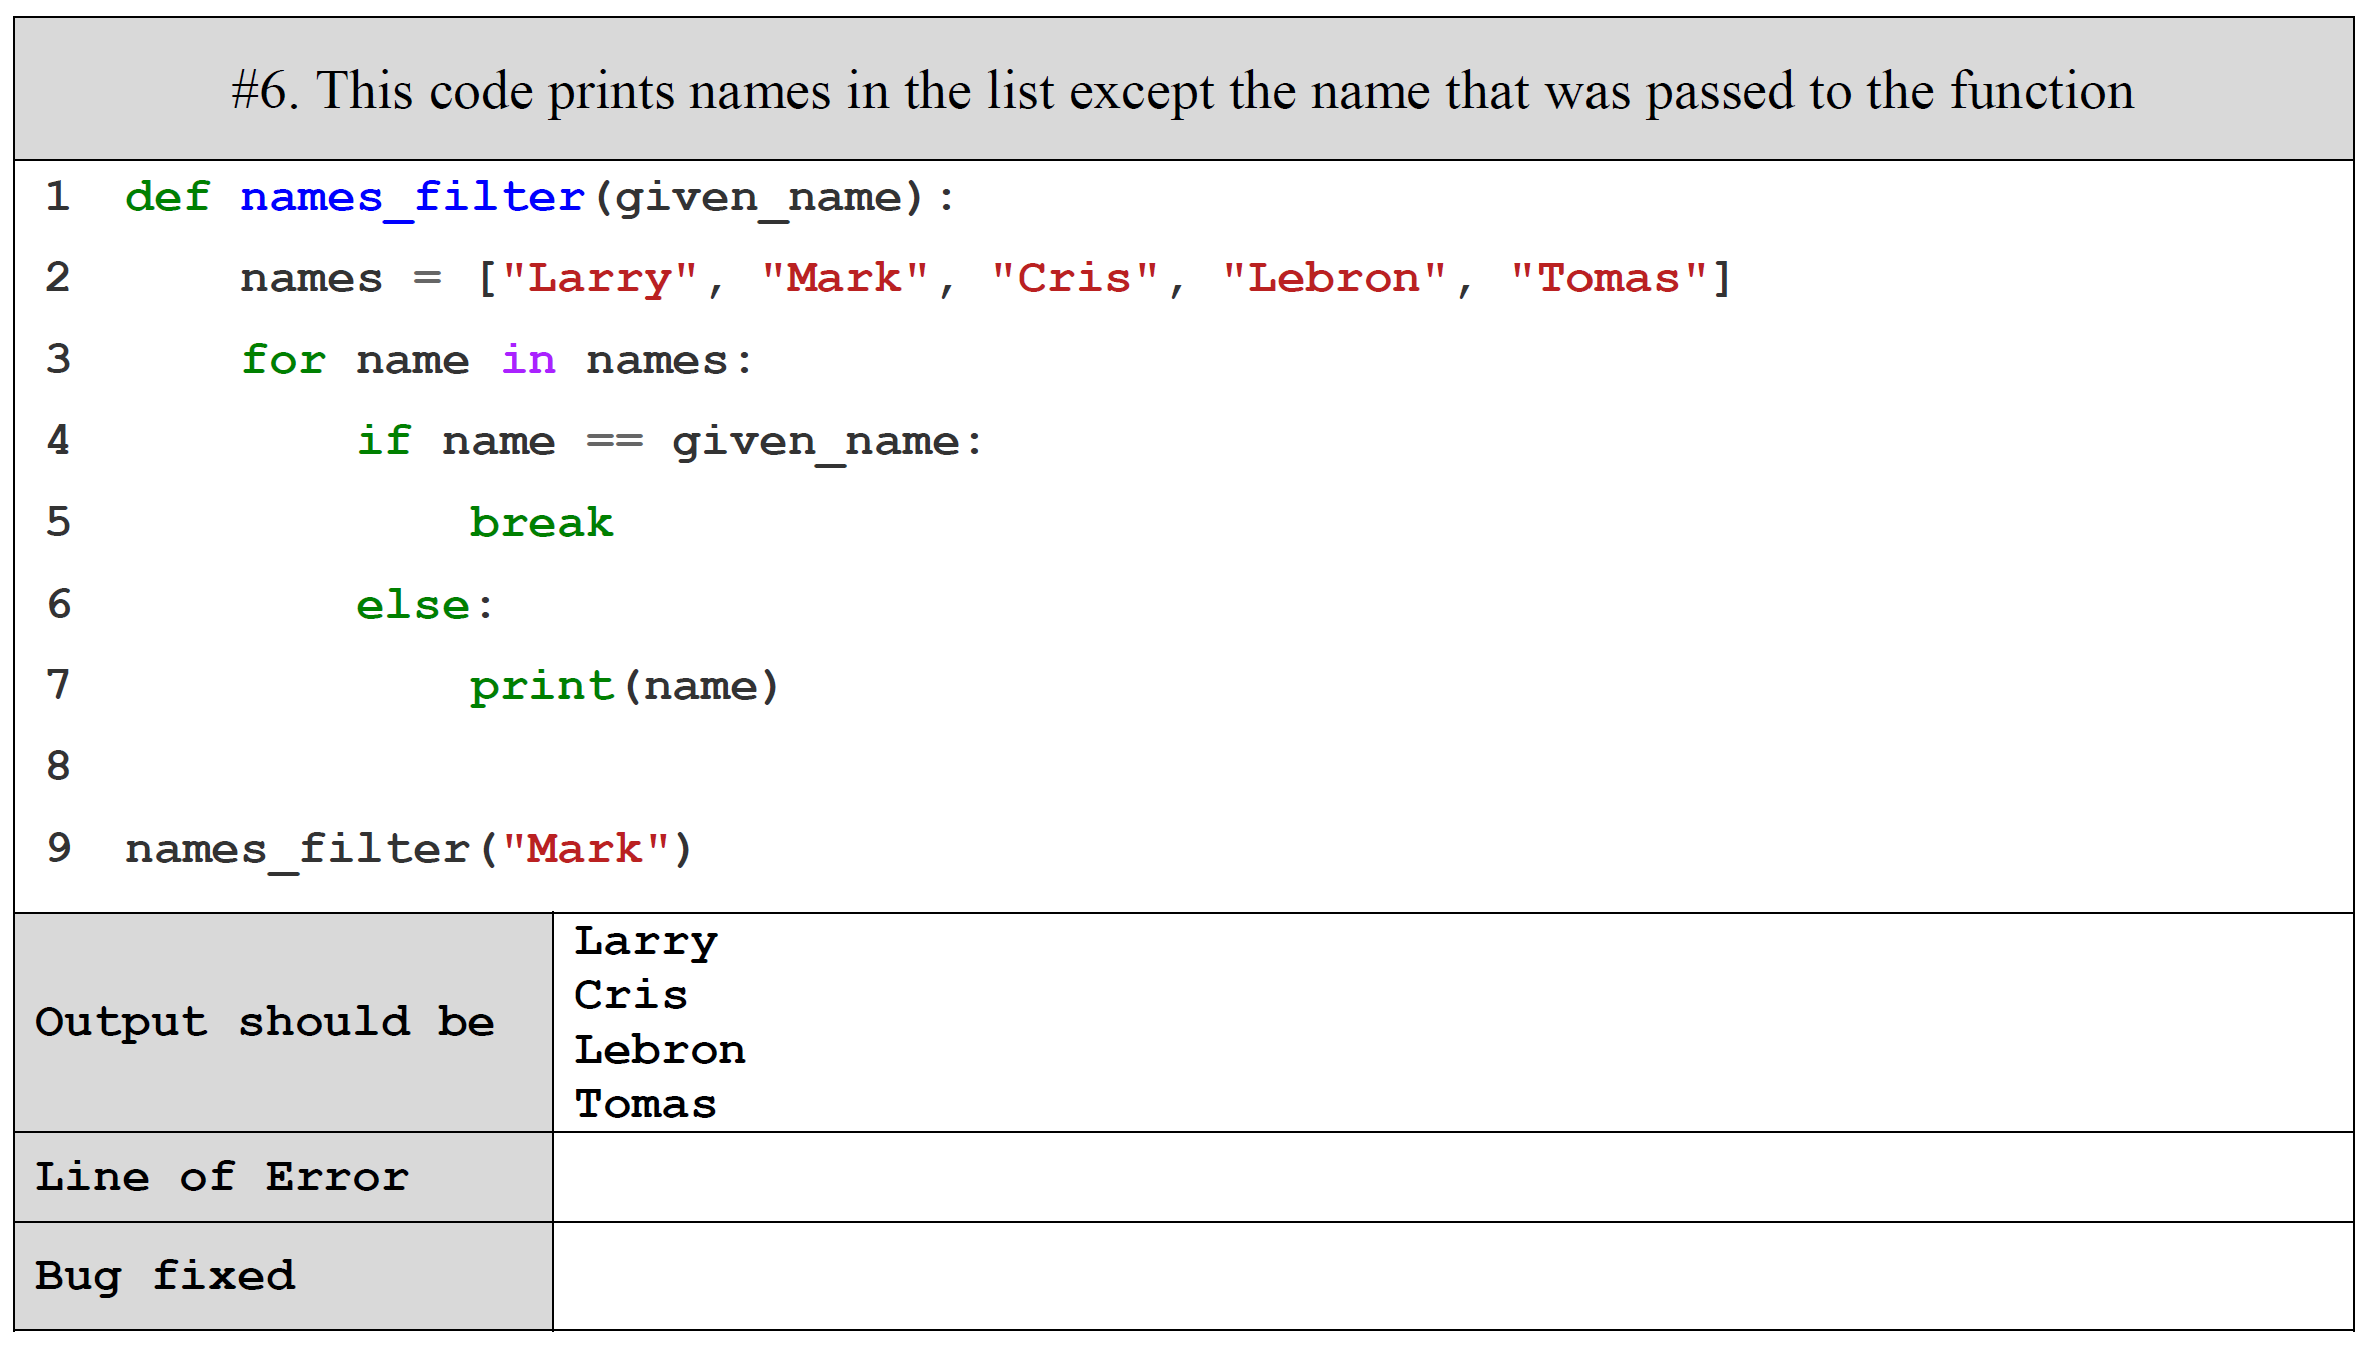
\includegraphics[width=\textwidth]{241_1.png}}
\caption{Question sample.}
\label{problemSample}
\end{figure}


\subsection{Bug Battles Competition}
Bug Battles which is a team-based competition was held in a classroom. The competition was held outside of class hours and it took place in eight separate sessions at varying times each day over the span of two weeks. The participants were divided into teams and each team has 4 members.
Each team was given 18 questions (6 for each programming language) that contain zero to one bug. Each question includes a short problem description, a buggy code, the code's output, a field to enter the line of error, and a bug fixed field to enter the correction of error as shown in Figure \ref{problemSample}. Each team has to find the bug in each question (if any) and write the line number of the error and how to fix it. Participants have to cover all the statements of the buggy code to detect any errors. In case there is no error or participants do not know the answer, they write ``0'' in the line number of error and ``Do not know'' in the bug fixed field. Each team receives points for the number of bugs that they catch and fix. 

\subsection{Post-survey}
The post-survey was conducted after the Bug Battles competition to collect individual opinions about the Bug Battles experience. The survey is based on a five-point likert scale that captures respondents' level of agreement: Strongly disagree, Disagree, Neutral, Agree, and Strongly agree \cite{weijters2021extremity}. The main goal of the post-survey is to answer the following research questions based on the participants' responses:
\begin{itemize}
   \item RQ1: Do Bug Battles increase participants' software testing skills?
   \item RQ2: Do Bug Battles encourage participants to learn new programming languages?
 \end{itemize}

\section{Results}
\label{section:results}
The post-survey results indicated that more than 93\% of the participants strongly agreed or agreed that detecting bugs with different programming languages enhances their software testing skills. On the other hand, less than 3\% of the participants strongly disagreed or disagreed while less than 4\% were neutral as shown in Figure \ref{fig:q.a}.
It is important to note that these positive responses prove how competitions might improve software testing skills. These findings are consistent with previous research in terms of improving software testing skills after experiencing the competition \cite{bryce2013bug}.  
\begin{figure}[!h]
{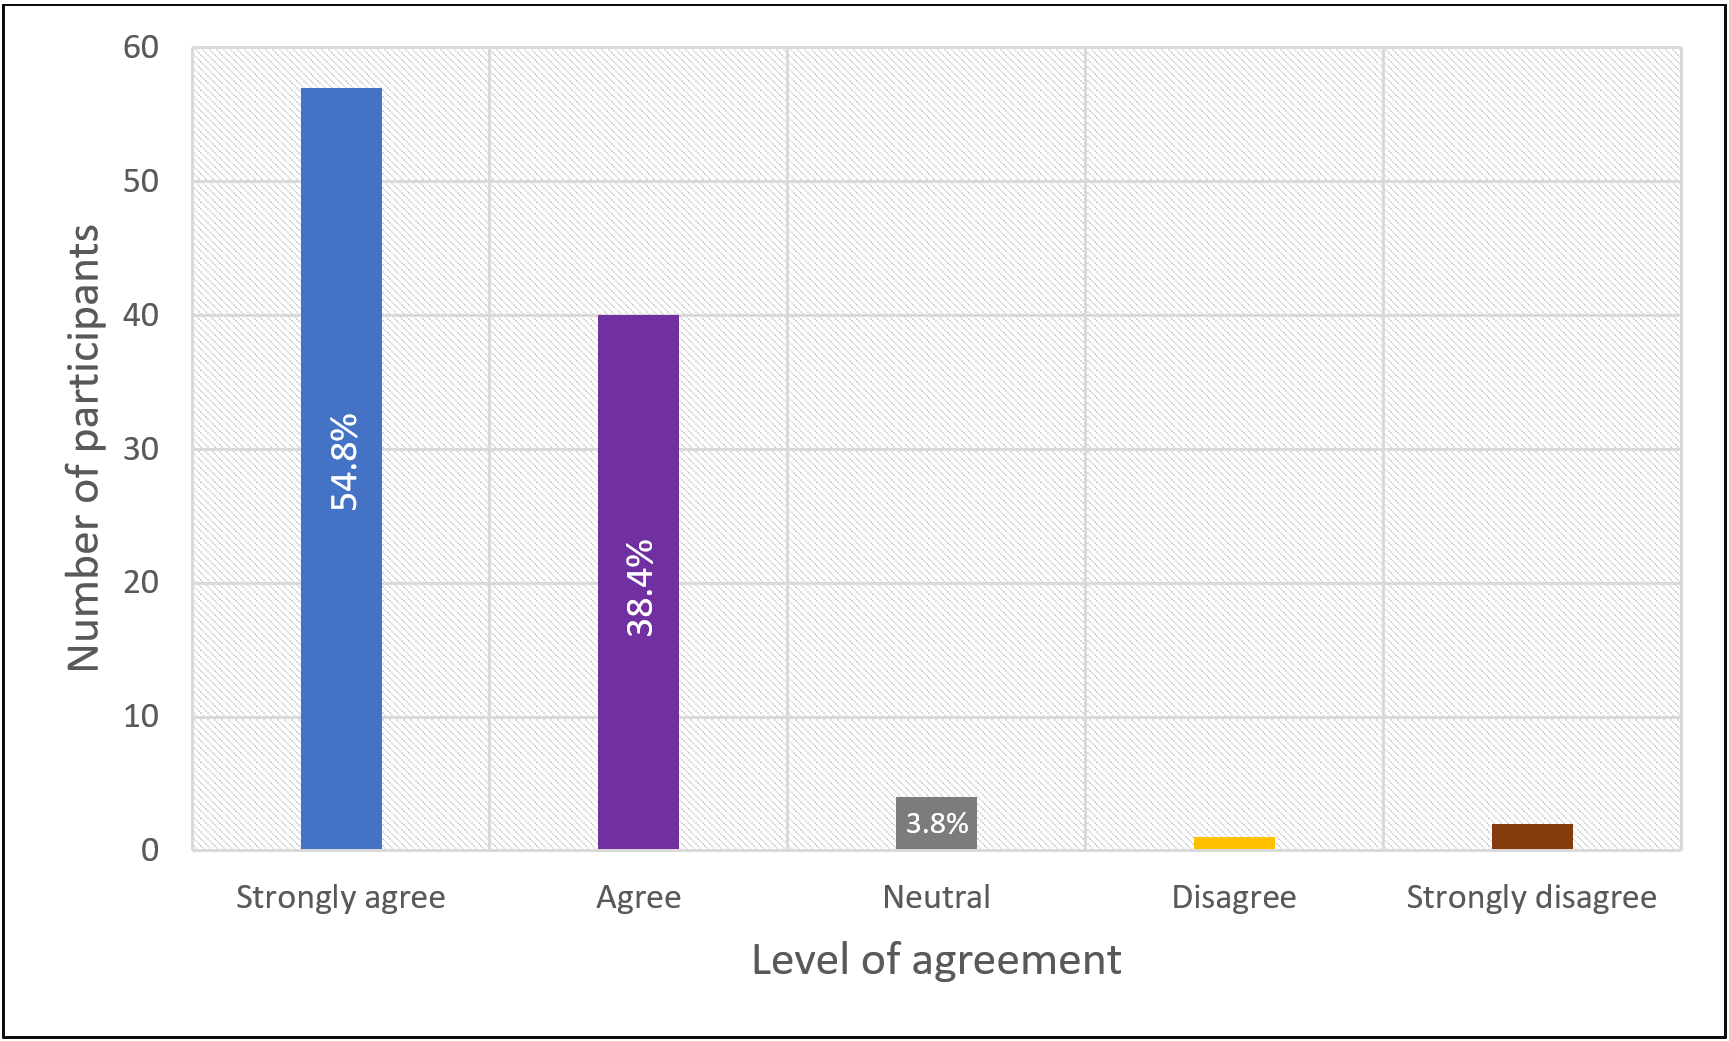
\includegraphics[width=\textwidth]{241_2.png}}
\caption{Result of increasing software testing skills.} \label{fig:q.a}
\end{figure}

Figure \ref{fig:q.b} presents that 93.26\% of participants agreed or strongly agreed that competition like this motivates them to learn more programming languages. This result is not surprising to us since some students were new to one or more languages in the competition. Another explanation for this result is using different programming languages in the competition and these languages were included based on their preferences. It is noteworthy that none of the participants disagreed, while only 2 expressed strong disagreement. 
\begin{figure}[!h]
{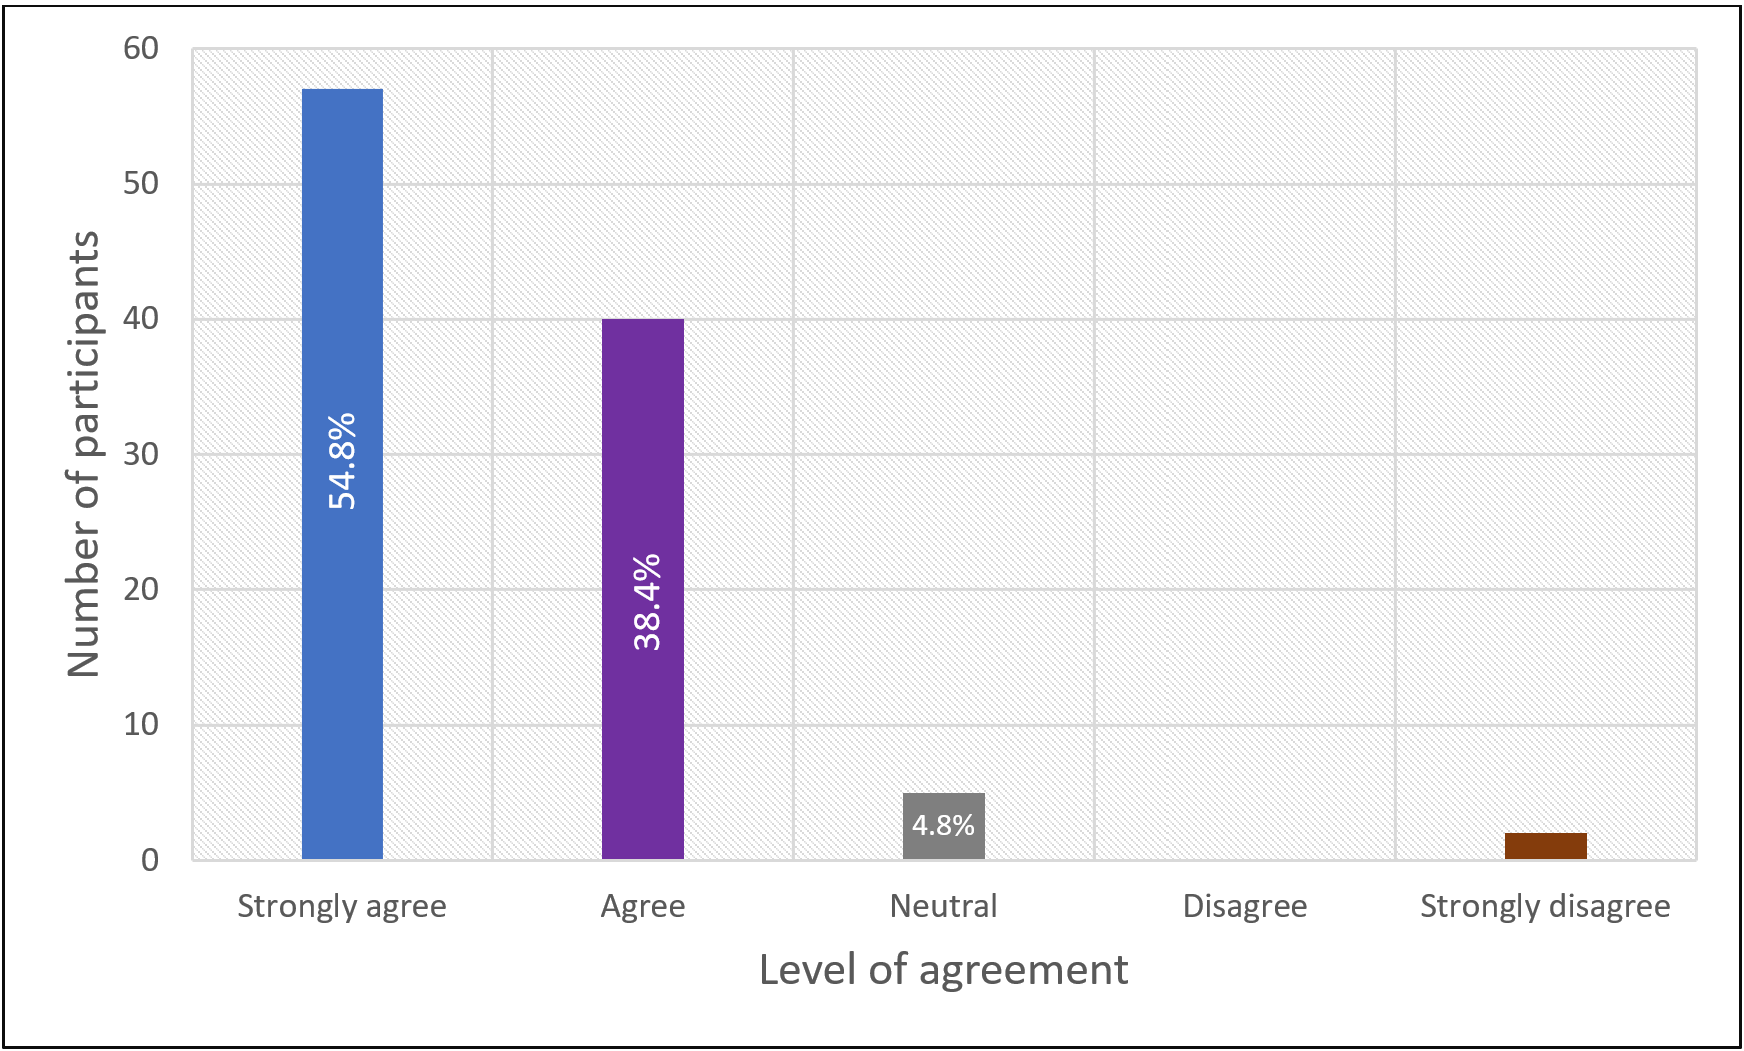
\includegraphics[width=\textwidth]{241_3.png}}
\caption{Result of increasing motivation to learn new programming languages.} \label{fig:q.b}
\end{figure}

The vast majority of the participants believed that their skills were improved to compare programming languages' syntax. Some participants did not know that they do not need to declare the type of variables in some languages like Python, as they do in Java or C++. The Python problems set helped them to discover the nature of the dynamic programming language.  More than 80\% of the participants preferred working in teams rather than working individually to catch bugs.  In contrast, a tiny minority of the participants who disagreed or strongly disagreed to work in teams with approximately less than 2\%. The participants shared their points of view regarding the excitement of Bug Battles and whether it motivated them to join future bug-catching competitions. The results showed that a high percentage of the participants found Bug Battles to be thrilling and beneficial. Additionally, 87.5\% of the participants either agreed or strongly agreed that Bug Battles had inspired them to participate in finding bugs competitions in the future. Figure \ref{fig:q.others} shows all the results in this paragraph.  

The findings of our research have implications for instructors as they can be used to improve their students' software testing skills and motivate them to learn new languages by holding team-based competitions. Additionally, these findings can have implications for software engineers as they can provide an opportunity for engineers to learn new languages and practice finding bugs. When participating in team-based competitions, engineers may encounter bugs and errors that they have never encountered before, which can provide a valuable learning opportunity to expand their software testing skill set. Moreover, in team-based competitions, engineers may have a learning experience as they communicate and collaborate with their team members in order to find and fix bugs.

\begin{figure}[htbp]
{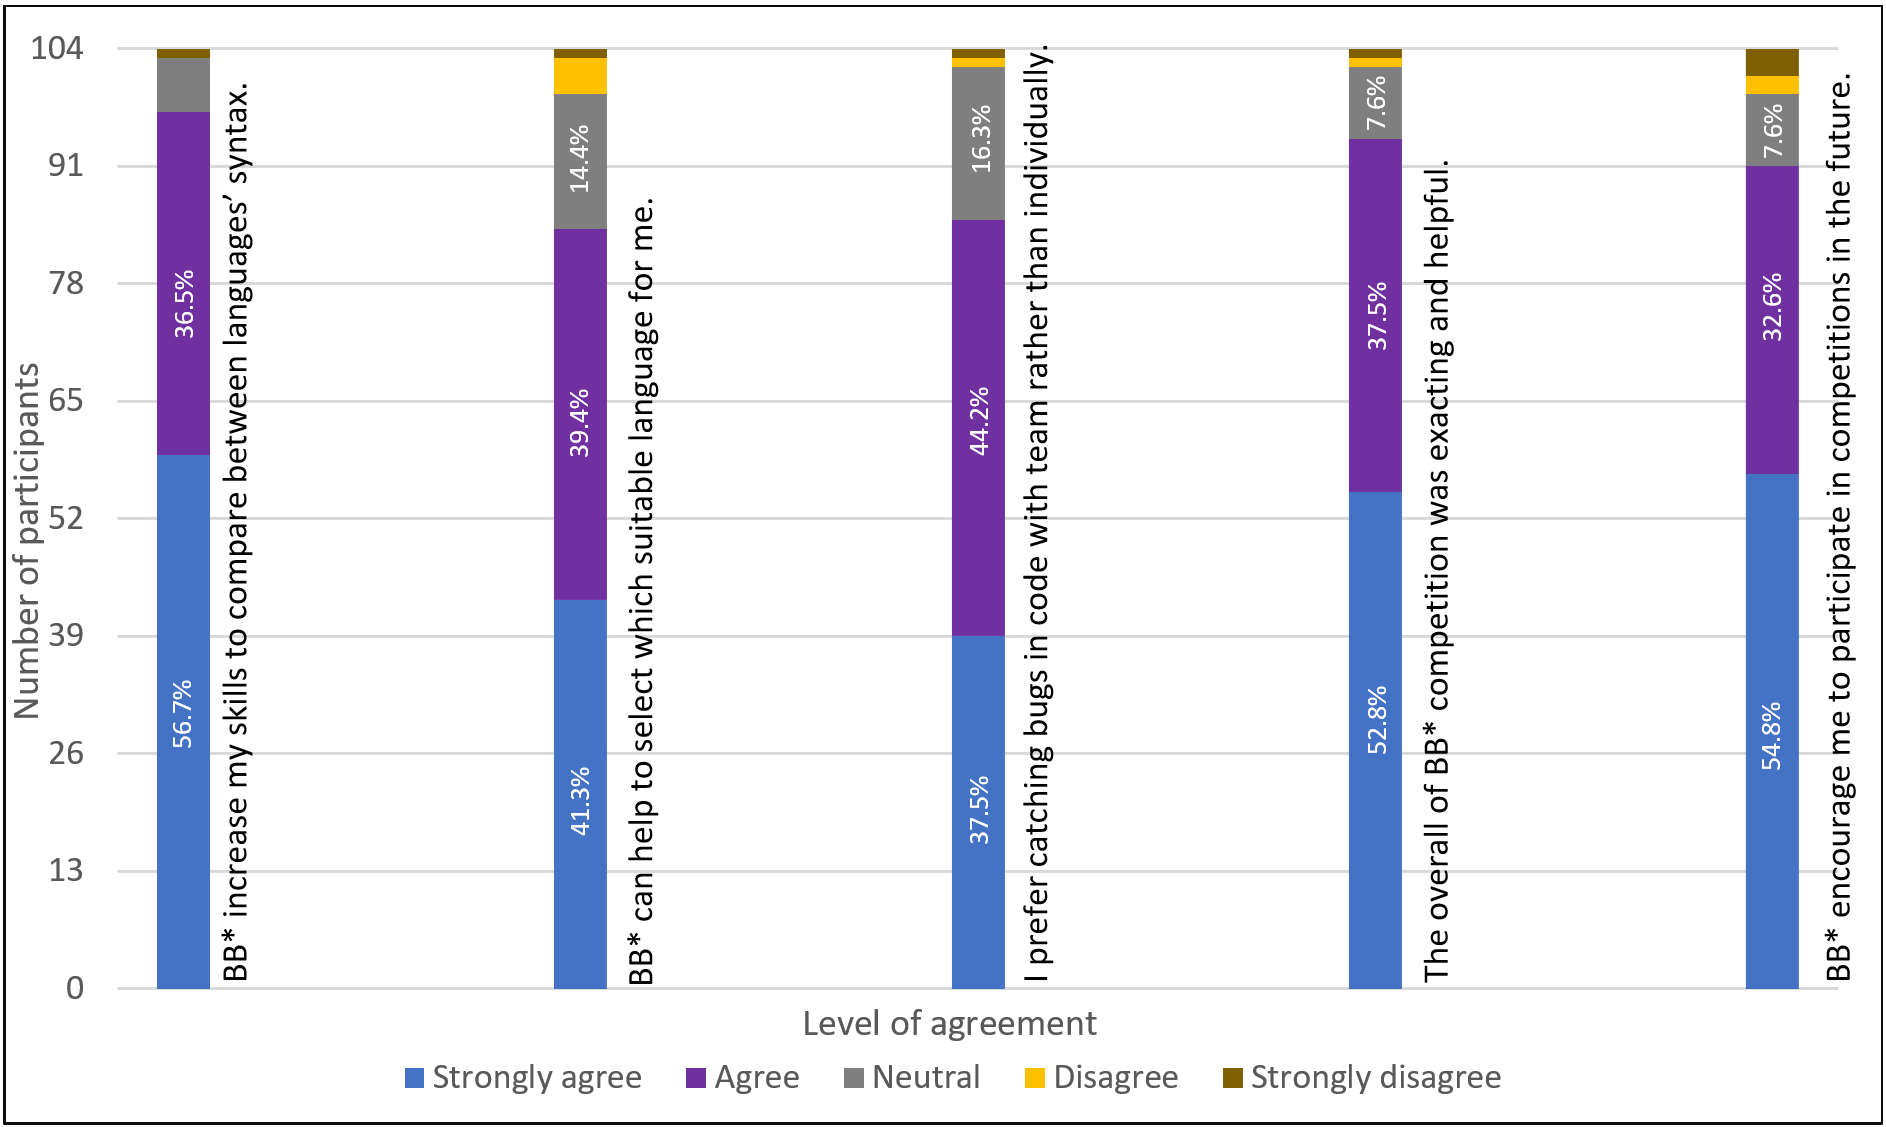
\includegraphics[width=\textwidth]{241_4.png}}
\footnotesize{ Note: *BB = Bug Battles}
\caption{Results of the other post-survey questions.} \label{fig:q.others}

\end{figure} 

\section{Threats to Validity} \label{section:threats} 
There are factors in our study that prevent us from generalizing the results to all students. We tried to minimize this risk by reaching 104 students. Another threat to validity is that different coding problems and bugs may change the results. We tried to minimize this risk by using 18 problems in the competition (six per programming language) and including bugs that we categorized as beginner, intermediate, and advanced in order to engage students. 



\section{Conclusion and Future Work} \label{section:conclusions}
Bug Battles is a team based competition in which teams compete to catch the most bugs in problem sets written in Python, Java, and C++. These languages were selected by the students in a pre-survey in an effort to include both familiar and new languages for the students. The results of the survey demonstrate that students have positive feelings toward Bug Battles in terms of motivating them to learn new languages and improving their software testing skills. We recommend instructors of computer programming courses organize team-based competitions to assist students in enhancing their software testing skills and inspire them to learn new programming languages. Problem sets and solutions may be freely downloaded from GitHub:\\
\url{https://github.com/Waleed9549/bugBattles}

Future work will examine Bug Battles competitions with more programming languages and problem sets. We plan to conduct a student focus group to develop problem sets based on bugs that focus group participants have encountered in different programming languages. We plan to solicit feedback from instructors and teach assistants about bugs that they notice their students encounter in an effort for us to include common bugs in Bug Battles. We hypothesize that customizing competitions to issues encountered by students will help students succeed in our programs.



\medskip
\bibliographystyle{plain}
\bibliography{241}

\end{document}
